\documentclass{article}

% Language setting
% Replace `english' with e.g. `spanish' to change the document language
\usepackage[english]{babel}
\usepackage{listings}
\usepackage{xcolor}
\usepackage{minted}

\lstset{ 
  backgroundcolor=\color{white},   % choose the background color; you must add \usepackage{color} or \usepackage{xcolor}; should come as last argument
  basicstyle=\footnotesize,        % the size of the fonts that are used for the code
  breakatwhitespace=false,         % sets if automatic breaks should only happen at whitespace
  breaklines=true,                 % sets automatic line breaking
  captionpos=b,                    % sets the caption-position to bottom
  commentstyle=\color{mygreen},    % comment style
  deletekeywords={...},            % if you want to delete keywords from the given language
  escapeinside={\%*}{*)},          % if you want to add LaTeX within your code
  extendedchars=true,              % lets you use non-ASCII characters; for 8-bits encodings only, does not work with UTF-8
  firstnumber=1000,                % start line enumeration with line 1000
  frame=single,	                   % adds a frame around the code
  keepspaces=true,                 % keeps spaces in text, useful for keeping indentation of code (possibly needs columns=flexible)
  keywordstyle=\color{blue},       % keyword style
  language=Octave,                 % the language of the code
  morekeywords={*,...},            % if you want to add more keywords to the set
  numbers=left,                    % where to put the line-numbers; possible values are (none, left, right)
  numbersep=5pt,                   % how far the line-numbers are from the code
  numberstyle=\tiny\color{mygray}, % the style that is used for the line-numbers
  rulecolor=\color{black},         % if not set, the frame-color may be changed on line-breaks within not-black text (e.g. comments (green here))
  showspaces=false,                % show spaces everywhere adding particular underscores; it overrides 'showstringspaces'
  showstringspaces=false,          % underline spaces within strings only
  showtabs=false,                  % show tabs within strings adding particular underscores
  stepnumber=2,                    % the step between two line-numbers. If it's 1, each line will be numbered
  stringstyle=\color{mymauve},     % string literal style
  tabsize=2,	                   % sets default tabsize to 2 spaces
  title=\lstname                   % show the filename of files included with \lstinputlisting; also try caption instead of title
}


\usepackage[letterpaper,top=2cm,bottom=2cm,left=3cm,right=3cm,marginparwidth=1.75cm]{geometry}

% Useful packages
\usepackage{amsmath}
\usepackage{graphicx}
\usepackage[colorlinks=true, allcolors=blue]{hyperref}
\usepackage{subfig}

\title{Projet Reseau}
\author{Nathan Seignole Mathis Vermeren}

\begin{document}
\maketitle

\begin{abstract}
Your abstract.
\end{abstract}

\section{Introduction}

Your introduction goes here! 

\section{Mise en place avec le protocole TCP}

\subsection{Initialisation de la connnexion}
Le programme commence par une fonction \mintinline{c}{void init(void)} qui nous sert juste à rendre le code compatible avec windows avec : \mintinline{c}{WSAStartup(MAKEWORD(2, 2), &wsa);}. Elle permet d'initialiser une DLL permettant d'utiliser les sockets. Pareillement, \mintinline{c}{void end(void)} permet de libérer cette même DLL avec \mintinline{c}{WSACleanup();}.

On entre ensuite dans \mintinline{c}{int init_connection(int PORT)}, elle crée un socket, configure son adresse et son port, le lie à l'adresse et au port spécifiés, puis le met en mode écoute pour accepter les connexions entrantes.
On créer le socket : 

\begin{minted}{c}
   SOCKET sock = socket(AF_INET, SOCK_STREAM, 0);
\end{minted}
On utilise un protocoles internet IPV4 (AF\_INET), SOCK\_STREAM est un type de communication, et 0 correspond au protocol par défaut. 

La structure \mintinline{c}{sockaddr_in} (sin) est configurée pour spécifier l'adresse IP et le port auquel le serveur sera lié.

Configuration de la Structure \mintinline{c}{sockaddr_in} :

\begin{minted}{c}
   sin.sin_addr.s_addr = htonl(INADDR_ANY);
   sin.sin_port = htons(PORT);
   sin.sin_family = AF_INET;
\end{minted}

- \mintinline{c}{sin.sin_addr.s_addr} : L'adresse IP est configurée en utilisant \mintinline{c}{htonl} pour convertir l'adresse IP en format réseau.
- \mintinline{c}{sin.sin_port} : Le numéro de port est configuré en utilisant \mintinline{c}{htons} pour convertir le numéro de port en format réseau.
- \mintinline{c}{sin.sin_family} : La famille d'adresses est spécifiée comme étant IPv4.

\subsubsection*{Liaison du Socket}

\begin{minted}{c}
   bind(sock, (SOCKADDR *) &sin, sizeof sin);
\end{minted}

Cette étape associe une adresse IP et un numéro de port au socket créé.

\subsubsection*{Mise en Mode Écoute}

\begin{minted}{c}
   listen(sock, MAX_CLIENTS);
\end{minted}

Le socket est mis en mode écoute pour accepter les connexions entrantes, avec \mintinline{c}{MAX_CLIENTS} spécifiant le nombre maximal de connexions en attente dans la file d'attente.

Ainsi, la fonction \mintinline{c}{init_connection} crée un socket, configure son adresse et son port, le lie à l'adresse et au port spécifiés, puis le met en mode écoute pour accepter les connexions entrantes.

\subsection{Fonctions clées}
\subsubsection*{\mintinline{c}{send} : }
La fonction \mintinline{c}{send} est utilisée dans la fonction \mintinline{c}{write_client} pour envoyer des données à un client connecté. 
\begin{minted}{c}
send(sock, buffer, strlen(buffer), 0)
\end{minted}
Elle envoie les données du tampon \mintinline{c}{buffer} sur le socket spécifié par \mintinline{c}{sock}. 0 est un indicateurs (\mintinline{c}{flags}) spécifiant le comportement de l'envoi. La fonction retourne le nombre d'octets envoyés en cas de succès, et -1 en cas d'erreur.

\subsubsection*{\mintinline{c}{accept} : }
La fonction \mintinline{c}{accept} est utilisée pour accepter une nouvelle connexion sur un socket. Dans \mintinline{c}{app} on écrit : 
\begin{minted}{c}
int csock = accept(sock, (SOCKADDR *)&csin, &sinsize);
\end{minted}
utilise la fonction \mintinline{c}{accept} pour accepter une nouvelle connexion sur le socket \mintinline{c}{sock}. Elle crée un nouveau descripteur de fichier de socket \mintinline{c}{csock} pour la nouvelle connexion. La structure \mintinline{c}{csin} est utilisée pour stocker l'adresse du client, et \mintinline{c}{sinsize} est un pointeur vers la taille de cette structure. Après l'appel à \mintinline{c}{accept}, \mintinline{c}{csock} contient le descripteur de fichier du nouveau socket connecté.


\begin{figure}[h]
    \hspace*{-2cm}  
    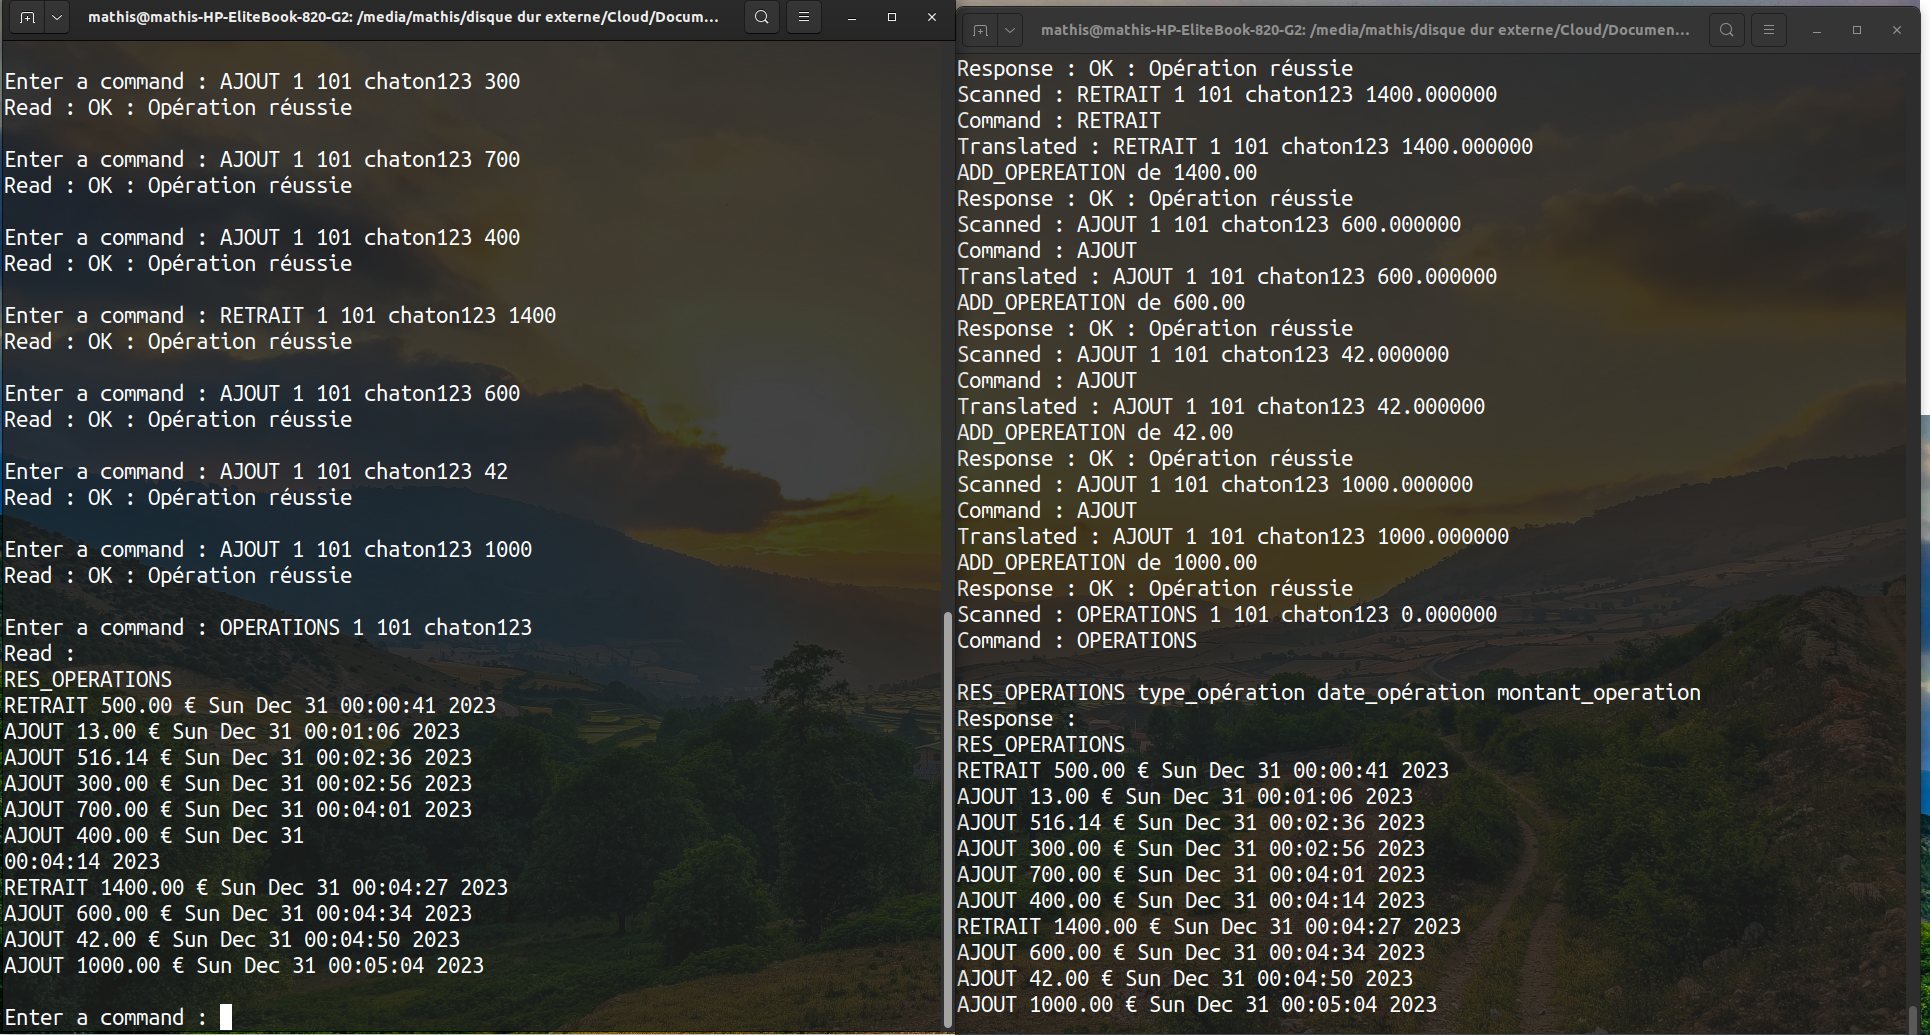
\includegraphics[width=1.25\linewidth]{OPERATIONS_TCP.png}
    \caption{\label{fig:OPERATIONS_TCP}Seulement 10 opérations s'affichent.}
\end{figure}

\begin{figure}[h]
    \hspace*{-2cm}  
    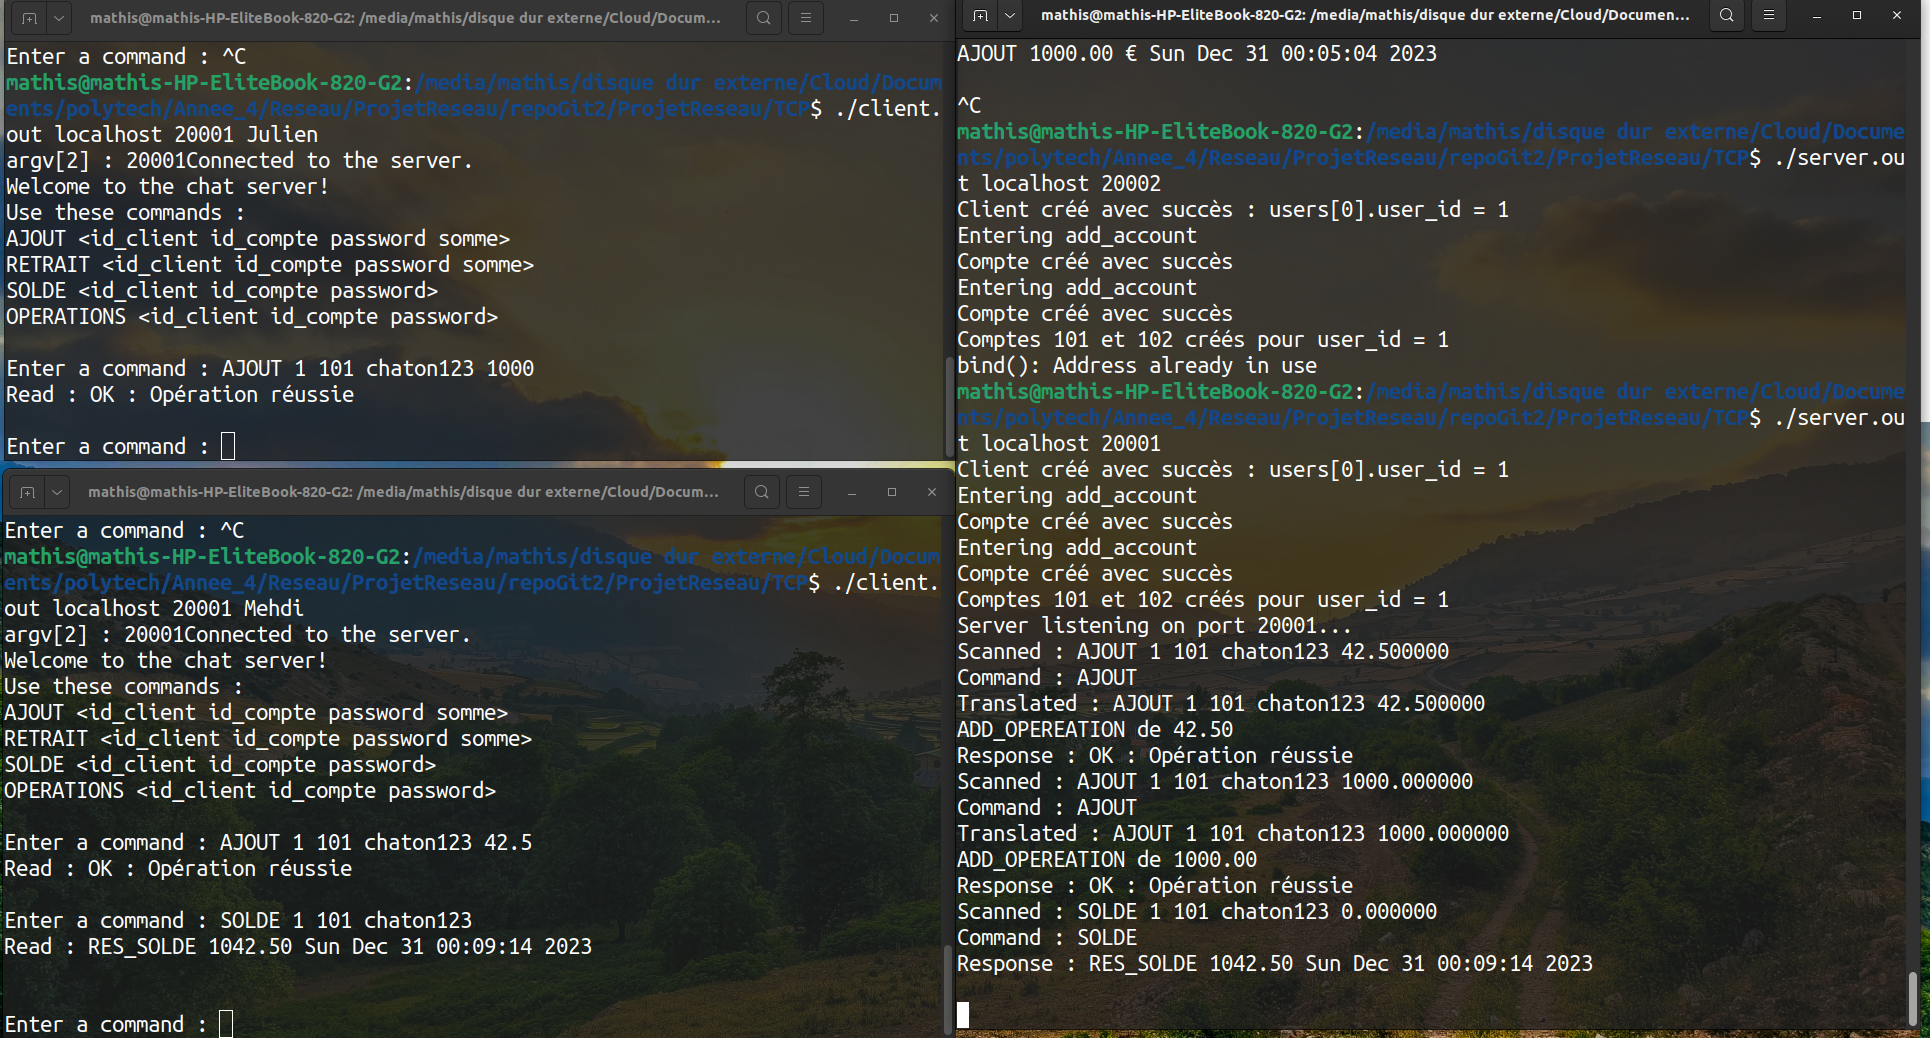
\includegraphics[width=1.25\linewidth]{TCPmultiClients.png}
    \caption{\label{fig:TCPmultiClients}Le TCP Fonctionne bien en Multi-Clients}
\end{figure}

\begin{figure}[h]
   \hspace*{-2cm}  
   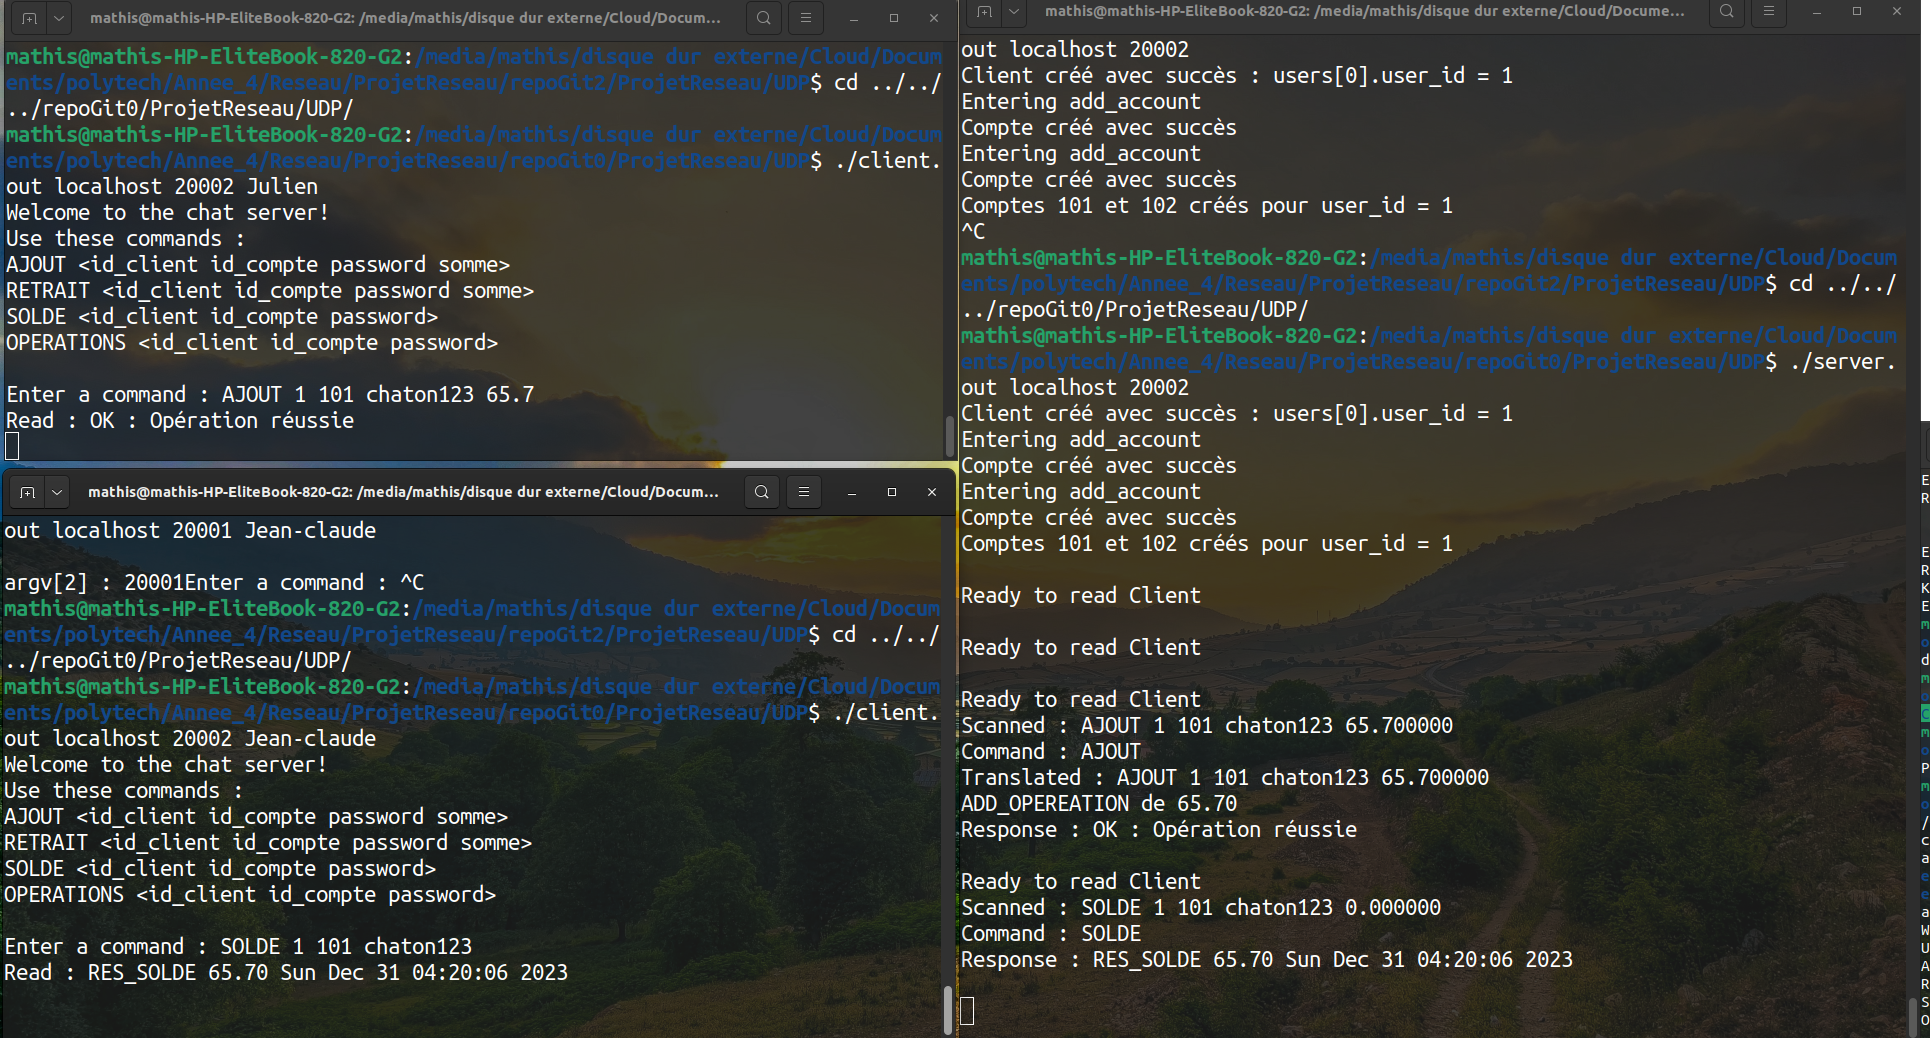
\includegraphics[width=1.25\linewidth]{UDPmultiClients.png}
   \caption{\label{fig:UDPmultiClients}Le UDP Fonctionne bien en Multi-Clients}
\end{figure}

\end{document}
